% \newpage
% \onecolumn

\appendices

\section{Censys queries}
\label{appendix:censys_queries}

The queries used to retrieve hosts from Censys are shown below. One command was used for each protocol. Note that the number of pages used was large enough to fetch all hosts from Censys. Alternatively, one could set the ``pages'' flag to $-1 $ to retrieve all the pages.

% \lstset{
%   language=bash, 
%   basicstyle=\ttfamily\small,
%   keywordstyle=\color{blue},
%   commentstyle=\color{gray},
%   stringstyle=\color{black},
%   numbers=left,
%   numberstyle=\tiny\color{gray},
%   stepnumber=1,
%   numbersep=5pt,
%   backgroundcolor=\color{white},
%   frame=single,
%   breaklines=true,
%   breakatwhitespace=false,
%   showspaces=false,
%   showstringspaces=false,
% }

\definecolor{mygreen}{rgb}{0,0.6,0}
\definecolor{mygray}{rgb}{0.5,0.5,0.5}
\definecolor{myblue}{rgb}{0,0,0.8}
\definecolor{myorange}{rgb}{0.8,0.4,0}

% Define style for shell scripts
\lstdefinestyle{shellstyle}{
    backgroundcolor=\color{white},   
    commentstyle=\color{mygreen},
    keywordstyle=\color{myblue},
    numberstyle=\tiny\color{mygray},
    stringstyle=\color{myorange},
    basicstyle=\ttfamily\footnotesize,
    breakatwhitespace=false,         
    breaklines=true,                 
    captionpos=b,                    
    keepspaces=true,                 
    numbers=left,                    
    numbersep=5pt,                  
    showspaces=false,                
    showstringspaces=false,
    showtabs=false,                  
    tabsize=2,
    language=bash
}

% Define colors for syntax highlighting
\definecolor{mygreen}{rgb}{0,0.6,0}
\definecolor{mygray}{rgb}{0.5,0.5,0.5}
\definecolor{mymauve}{rgb}{0.58,0,0.82}
\definecolor{myblue}{rgb}{0,0,0.8}

% Define style for Python listings
\lstdefinestyle{pythonstyle}{
    backgroundcolor=\color{white},   
    commentstyle=\color{mygreen},
    keywordstyle=\color{myblue},
    numberstyle=\tiny\color{mygray},
    stringstyle=\color{mymauve},
    basicstyle=\ttfamily\footnotesize,
    breakatwhitespace=false,         
    breaklines=true,                 
    captionpos=b,                    
    keepspaces=true,                 
    numbers=left,                    
    numbersep=5pt,                  
    showspaces=false,                
    showstringspaces=false,
    showtabs=false,                  
    tabsize=2,
    language=Python
}

% % Apply the style to Python listings
% \lstset{style=pythonstyle}

% Apply the style to shell listings
\lstset{style=shellstyle}

\begin{itemize}
\item DNS:
\begin{lstlisting}[language=bash, caption=DNS query., label=lst:censys_dns]
censys search 'services.service_name: DNS and services.port:53 and 
location.country: "Greece"' --per-page 100 --pages 77 > dns.json
\end{lstlisting}
\item NTP:
\begin{lstlisting}[language=bash, caption=NTP query., label=lst:censys_ntp]
censys search 'services.service_name: NTP and services.port:123 and 
location.country: "Greece"' --per-page 100 --pages 267 > ntp.json 
\end{lstlisting}
\item Memcached:
\begin{lstlisting}[language=bash, caption=Memcached query., label=lst:censys_memcached]
censys search 'services.service_name: MEMCACHED and services.port:11211 and  
location.country: "Greece"' --per-page 100 --pages 1 > memcached.json
\end{lstlisting}

\end{itemize}




\section{Filter queries}
\label{appendix:filter_queries}

After gathering our hosts, we send simple queries to each one to see whether or not they are open to the public in our so-called ``filtering'' stage. Each query strategy (i.e. hand-crafted packet) is shown below. For DNS, we send a simple ``A'' query to resolve the IP address of google.com, as demonstrated in Listing~\ref{lst:check_dns}. When filtering NTP hosts, we first send a normal Mode 3 (client) request that can be seen in Listing~\ref{lst:check_ntp_1} and then send a ``monlist'' packet to the servers that responded to the previous query, as shown in Listing~\ref{lst:check_ntp_2}. We send a ``stats slabs'' request for Memcached hosts to filter them, as shown in Listing~\ref{lst:check_memcached}.

\lstset{style=pythonstyle}

\begin{itemize}
\item DNS:
\begin{lstlisting}[language=python, caption=DNS ``A'' request., label=lst:check_dns]
pkt = IP(dst=ip) / UDP(dport=53, sport=RandShort()) / DNS(rd=1, qd=DNSQR(qname="google.com"))
\end{lstlisting}
\item NTP:
\begin{lstlisting}[language=python, caption=NTP request., label=lst:check_ntp_1]
pkt = IP(dst=ip) / UDP(dport=123, sport=RandShort()) / NTP(version=4, mode=3)
\end{lstlisting}
\begin{lstlisting}[language=python, caption=NTP ``monlist'' query., label=lst:check_ntp_2]
data = "\x17\x00\x03\x2a" + "\x00" * 4  
# 0x17 for private mode, 0x00 for response, 0x03 for version, 0x2a for monlist
pkt = (IP(dst=ip) / UDP(dport=123, sport=RandShort()) / Raw(load=data)) 
\end{lstlisting}
\item Memcached:
\begin{lstlisting}[language=python, caption=Memcached ``stats slabs'' request., label=lst:check_memcached]
pkt = IP(dst=ip) / UDP(sport=RandShort(), dport=11211) / Raw(load="\x00\x01\x00\x00\x00\x01\x00\x00stats slabs\r\n")
\end{lstlisting}

\end{itemize}




\section{Measurement queries}
\label{appendix:measurement_queries}

To measure the BAF for the protocols, we have hand-crafted different packets that will lead to high amplification. In the case of DNS, we send an ``ANY'' request to the ``.sl'' TLD, presented in Listing~\ref{lst:measure_dns}. Note from the code that the request can easily be changed to be a ``DNSKEY'' or ``RRSIG'' request by changing the ``query\_type'' accordingly. We have mostly tried ``ANY'' as it would lead to the highest amplification factor if the server responded to it. For NTP, we send a ``monlist'' request, which was presented in Listing~\ref{lst:check_ntp_2}, along with some other private Mode queries~\cite{rapid7_private}, that are shown in Listing~\ref{lst:measure_ntp_private}.  For Memcached, we need to send two initial queries to find information about the keys and values present in the server. Our first query is a ``stats items'' query (Listing~\ref{lst:measure_mem_1}). This command retrieves statistical information about the items stored in the cache, providing details about each slab class (a logical grouping of cache entries of similar size). We parse the output from this command to retrieve all slab IDs. We then send, for each slab ID, a ``stats cachedump'' request (Listing~\ref{lst:measure_mem_2}). The 0 in the request indicates no limit, i.e. the server should answer with all items. This query retrieves information about items stored in a specific slab class. Each entry (i.e. item) contains the key, the size of the associated value and a timestamp (when the item was last accessed or possibly when it was set, depending on the version and configuration). This is the information we were looking for as we look to find the key and value that would lead to the highest BAF for the request we are considering (i.e. ``get $<key>$''). The code for this request is shown in Listing~\ref{lst:measure_mem_3}.

We also wanted to analyse the maximum theoretical BAF for Memcached for the ``get $<key> <key> ... <key>$'' request. We created a function for the theoretical BAF, named $b$, shown in Equation~\eqref{eq:mem_baf}, where $k$ is the size of the key, $v$ is the size of the associated value, and $t$ is the number of times the key appears in the ``get'' request. As $t$ tends to infinity, the BAF becomes equal to $\frac{v}{k + 1}$, as shown in Equation~\ref{eq:limit}. In the ideal case, the key has the smallest size possible, one character (thus one byte), and the value the largest size possible, 1 MB (i.e. $10^6$ bytes). This means that the largest theoretical BAF for this request will tend to a value of $\frac{10^6}{1+1} =\frac{10^6}{2}=500k$. This should show that the size of the key and the value associated with it directly impact the BAF potential of Memcached. 


\begin{figure}[htpb]
    \footnotesize
    \begin{equation}
     b(k, v,t) = \frac{v \cdot t}{13 + t \cdot (k + 1)}
    \label{eq:mem_baf}
    \end{equation}
    
    \begin{equation}
    \lim_{t \to \infty} b(k, v, t) = \lim_{t \to \infty} \frac{v \cdot t}{13 + t \cdot (k + 1)} = \frac{v}{k + 1}
    \label{eq:limit}
    \end{equation}
\end{figure}

\begin{itemize}
\item DNS:
\begin{lstlisting}[language=python, caption=DNS ``ANY'' request on ``.sl''., label=lst:measure_dns]
dns = DNS(ad=1)
dns.qd = DNSQR(qname=domain, qtype=query_type, qclass="IN")  # query section
dns.ar = DNSRROPT(rclass=4096, z=1)  # additional records
request = IP(dst=ip) / UDP(dport=53, sport=RandShort()) / dns
\end{lstlisting}
\item NTP:
\begin{lstlisting}[language=python, caption=NTP private Mode requests., label=lst:measure_ntp_private]
packet = IP(dst=target_ip) / UDP(dport=123, sport=RandShort()) / NTPPrivate(
        response=0,  # i.e. this is a request
        more=0,  # not expecting multiple packets
        version=2,  # version number 2/3
        implementation=3,  # assuming XNTPD
        auth=0,  # no authentication
        mode=7,  # 6 => mode 6 (control) or mode 7 (private)
        seq=0,  # sequence number
        request_code=command_code, # 0 for PEER_LIST, 1 for PEER_LIST_SUM, 16 for GET_RESTRICT
        # mode 6 => 12 for CTL_OP_REQ_NONCE and 31 for UNSETTRAP
        err=0,
        nb_items=0,  # number of data items
        mbz=0,  # must be zero
        data_item_size=0,  # size of each data item
    )
\end{lstlisting}
\item Memcached:
\begin{lstlisting}[language=python, caption=Memcached ``stats items'' request., label=lst:measure_mem_1]
pkt = IP(dst=ip) / UDP(sport=RandShort(), dport=11211) / 
Raw(load="\x00\x01\x00\x00\x00\x01\x00\x00stats items\r\n")
\end{lstlisting}
\begin{lstlisting}[language=python, caption=Memcached ``stats cachedump'' request., label=lst:measure_mem_2]
pkt = IP(dst=ip) / UDP(sport=RandShort(), dport=11211) / 
Raw(load=f"\x00\x01\x00\x00\x00\x01\x00\x00stats cachedump {slab_id} 0\r\n")
\end{lstlisting}
\begin{lstlisting}[language=python, caption=Memcached ``get $<key>$'' request., label=lst:measure_mem_3]
pkt = IP(dst=ip) / UDP(sport=RandShort(), dport=11211) / 
Raw(load=f"\x00\x01\x00\x00\x00\x01\x00\x00get key\r\n")
\end{lstlisting}

\end{itemize}



% 48 DNSKEY
  



    % packet = IP(dst=target_ip) / UDP(dport=123, sport=RandShort()) / NTPPrivate(
    %     # rm_vn_mode=0x1B,
    %     response=0,  # This is a request
    %     more=0,  # Not expecting multiple packets
    %     version=2,  # Version number 2/3
    %     implementation=3,  # Assuming XNTPD
    %     auth=0,  # No authentication
    %     mode=7,  # 6 => mode 6 (control), or mode 7 (private)
    %     seq=0,  # Sequence number
    %     request_code=command_code,  # => 12 for CTL_OP_REQ_NONCE and 31 for UNSETTRAP
    %     err=0,
    %     nb_items=0,  # Number of data items
    %     mbz=0,  # Must be zero
    %     data_item_size=0,  # Size of each data item
    %     # data=(b'\x00' * 40)  # => ntpdc and ntpq add padding
        % )
\section{Collect metadata}
\label{appendix:collect_metadata}


To grasp the connection between certain factors and the BAF achieved by hosts, we had to augment our existing knowledge with some metadata. We had different procedures, the code of which is shown below. For DNS, we retrieved the product (e.g. RedHat) and vendor information (e.g. Enterprise Linux) from the JSON file already provided by Censys. To classify an NS as recursive or not, we used the code snippet in Listing~\ref{lst:check_recursive}, where we essentially try to resolve the IP of ``google.com'' by using a specific nameserver recursively by setting the recursive flag. Note that we also set a timeout of one second and do not consider a server to be recursive in case of an error or a timeout. To obtain authoritative name servers, we used the flipped approach. We don't use any nameserver, but for each Greek domain we gathered, we looked up its authoritative nameserver via the ``dig'' query shown in Listing~\ref{lst:ns_dig}. As a result, we get the authoritative NS domains, which we then map to IP addresses with a simple ``dig'' query, see Listing~\ref{lst:ns_find_ip}. Finally, we only keep the authoritative NS IP if it is located in Greece, which we check using the geolocation tool ``ipinfo''~\cite{ipinfo}; the code for this is shown in Listing~\ref{lst:ip_geoloc}. This outputs a JSON with various information, and we use the ``country'' attribute, which we match with ``GR''. 

We have obtained the DNS software run by hosts by using the ``fpdns'' command line utility tool~\cite{fpdns_kirei}. The code is presented in Listing~\ref{lst:fpdns_code}. We set a timeout of 20 seconds per each request. Note that ``fpdns'' is not a well-maintained tool and likely has trouble distinguishing between newer versions of DNS software. We count this as a limitation of our analysis.

For NTP, we have only gathered the system information (i.e. the operating system run by a host). We used the ``ntpq'' CLI utility tool, as described in~\cite{ntpq}. The code for this is shown in Listing~\ref{lst:ntpq_code}. We parse the output and retrieve the value for the ``system'' attribute. 

\lstset{style=shellstyle}

\begin{lstlisting}[language=bash, caption=Resolve the IP of google.com recursively, label=lst:check_recursive]
dig @<ip> google.com +rec +time=1
\end{lstlisting}


\begin{lstlisting}[language=bash, caption=Finds the authoritative nameservers of the placeholder domain. , label=lst:ns_dig]
dig <domain> NS +short
\end{lstlisting}


\begin{lstlisting}[language=bash, caption=Resolve the IP address of the authoritative nameserver domain. , label=lst:ns_find_ip]
dig +short <nameserver_domain>
\end{lstlisting}

\begin{lstlisting}[language=bash, caption=Find geolocation information about placeholder IP. , label=lst:ip_geoloc]
curl http://ipinfo.io/<ip_address>/json
\end{lstlisting}

\begin{lstlisting}[language=bash, caption=Find DNS software information about the placeholder host. , label=lst:fpdns_code]
fpdns -t 20 <ip_address>
\end{lstlisting}

\begin{lstlisting}[language=bash, caption=Find operating system ran by NTP host. , label=lst:ntpq_code]
ntpq -c rv <ip_address>
\end{lstlisting}


\begin{figure}[t]
    \centering
        \centering
        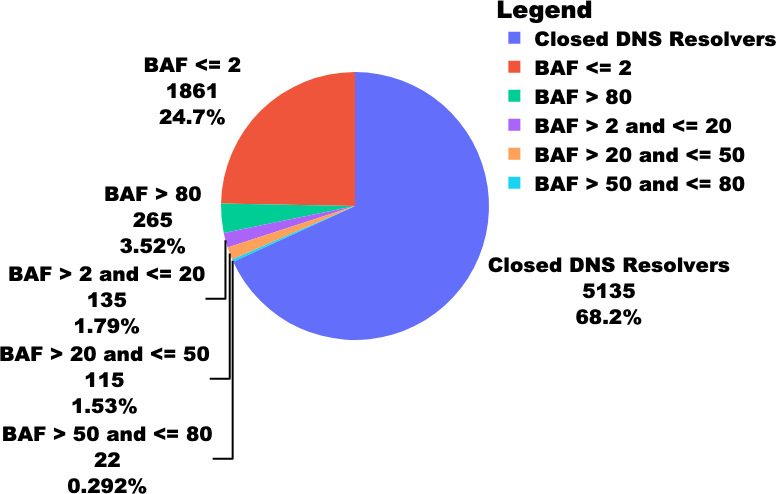
\includegraphics[width=0.48\textwidth]{research paper/plots/dns_sl_piechart_trim.png}
        \caption{DNS BAF distribution.}
        \label{fig:piechart_dns}
\end{figure}

\begin{figure}[t]
        \centering
        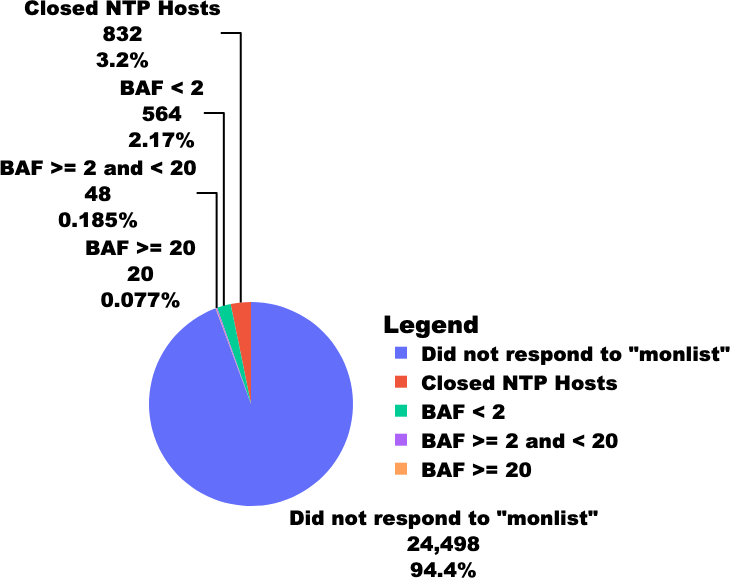
\includegraphics[width=0.48\textwidth]{research paper/plots/ntp_piechart_merged_trim.png}
        \caption{NTP BAF distribution.}
        \label{fig:piechart_ntp}
\end{figure}
    
\begin{figure}[t]
        \centering
        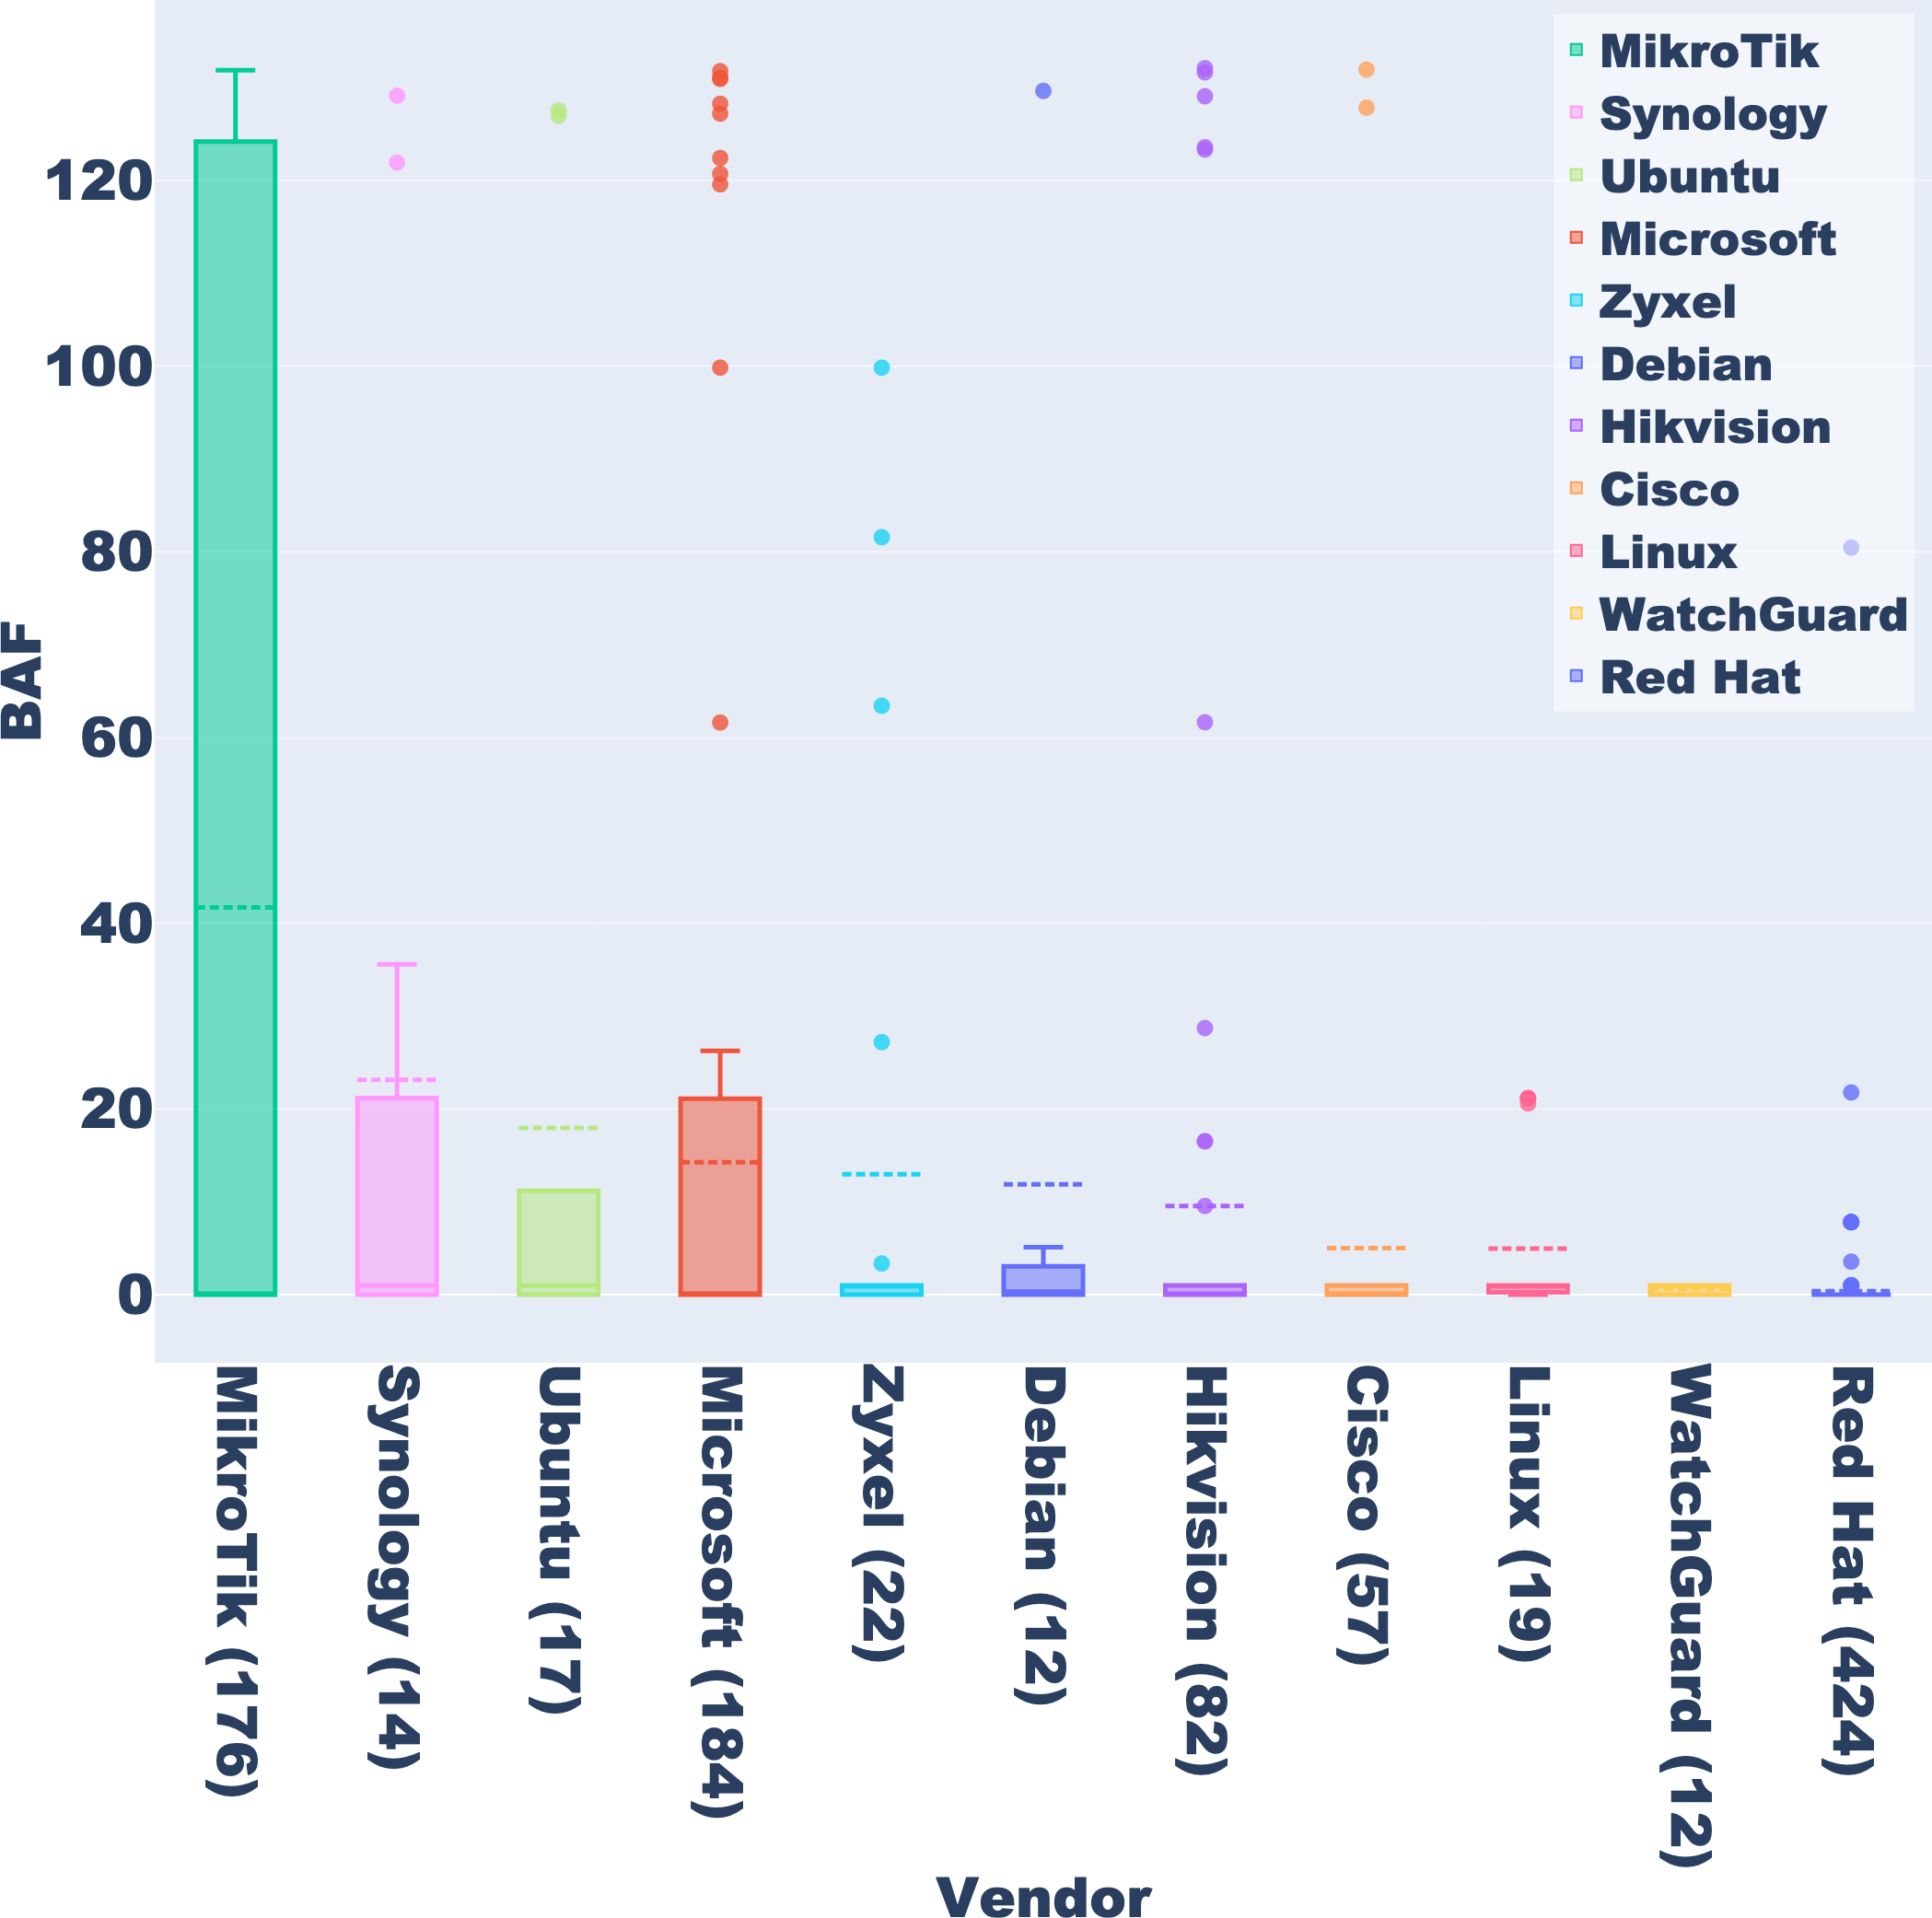
\includegraphics[width=0.48\textwidth]{research paper/plots/SL_vendor_boxplot_restricted_trim.png}
        \caption{Vendor against BAF (DNS).}
        \label{fig:boxplot_vendor}
\end{figure}
    
\begin{figure}[t]
        \centering
        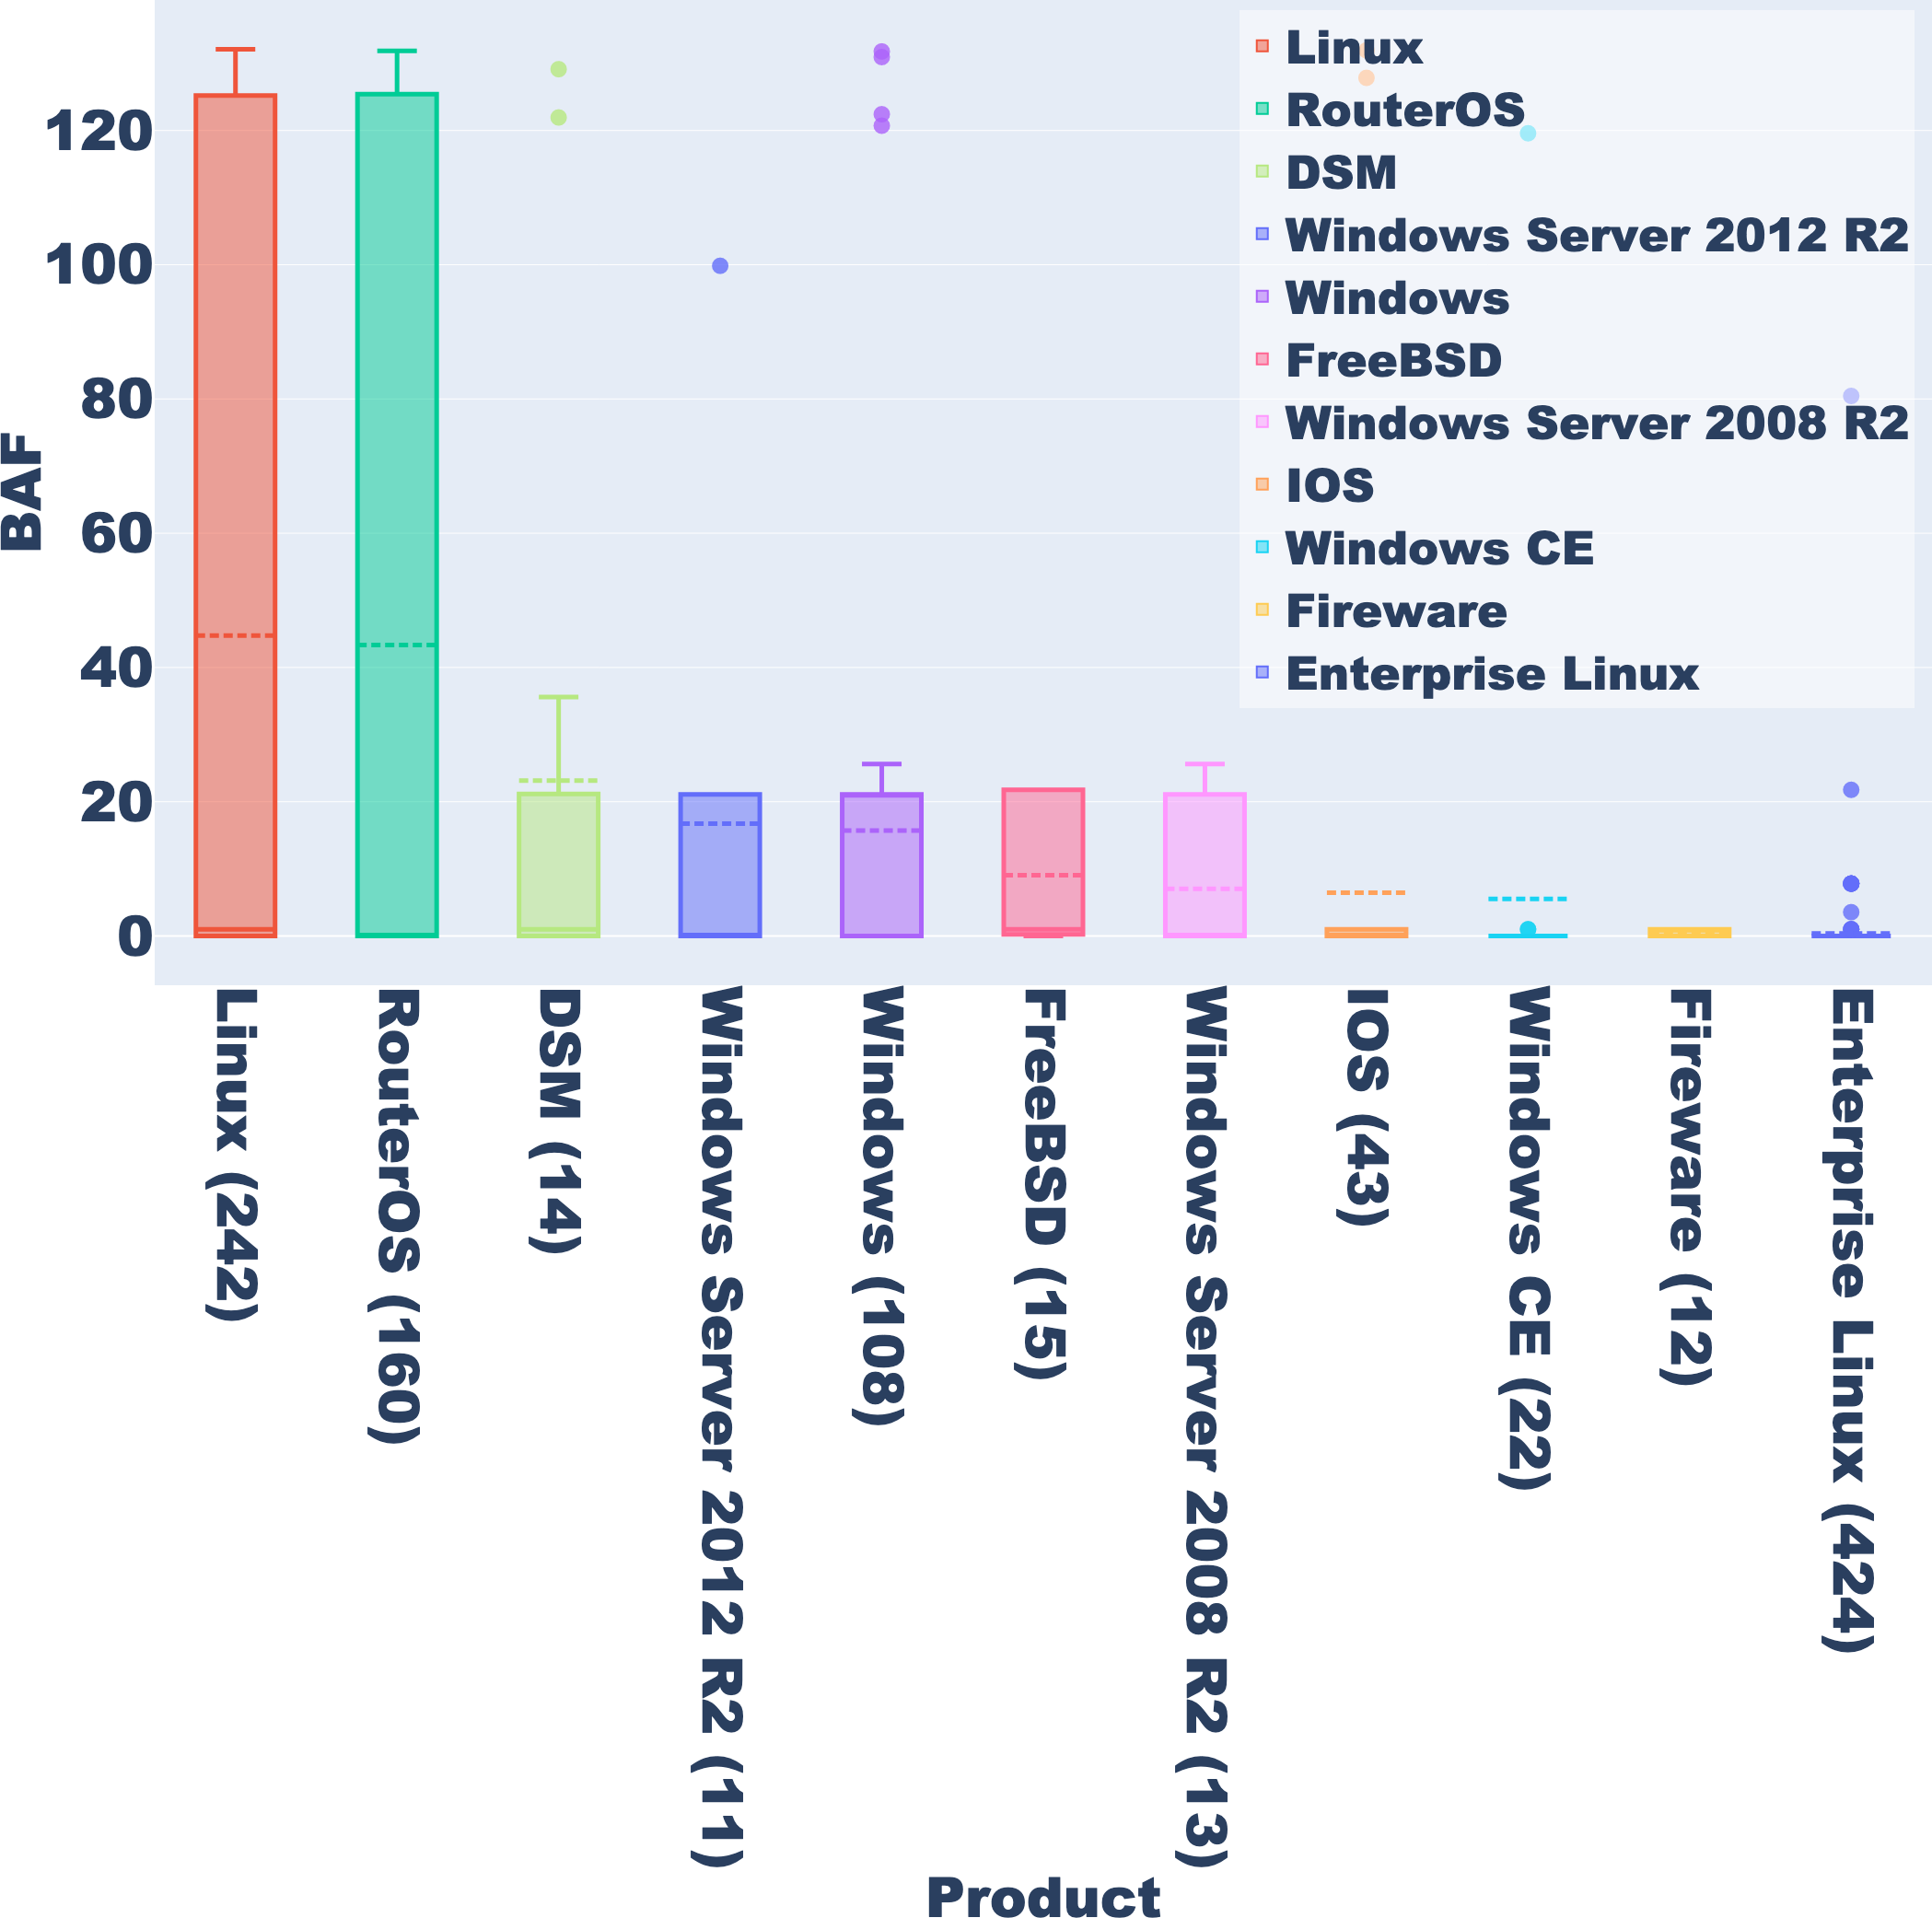
\includegraphics[width=0.48\textwidth]{research paper/plots/SL_product_boxplot_restricted_trim.png}
        \caption{Product against BAF (DNS).}
        \label{fig:boxplot_product}
\end{figure}
    % \caption{Piecharts for DNS and NTP and boxplots for DNS against product and vendor information.}
    % \label{fig:boxplots_piecharts}

\section{Piecharts and Boxplots}
\label{appendix:piecharts_boxplots}



The distribution of DNS hosts according to their BAF is shown in Fig.~\ref{fig:piechart_dns}. Most hosts are closed (68.2\%); however, quite a large amount of DNS hosts (265) achieve a BAF $\geq$ 80. A similar visualisation for NTP is shown in Fig.~\ref{fig:piechart_ntp}. Most NTP servers (94.4\%) did not respond to the ``monlist'' private Mode query for NTP. A few servers are closed (3.2\%), which was expected to ensure accurate and synchronised timekeeping across different devices and networks. Also, a tiny number (20) achieved a BAF $\geq 20$.  

The BAF distribution is depicted in a boxplot from the DNS hosts, whose vendor information we know, in Fig.~\ref{fig:boxplot_vendor}. Red Hat hosts are secure, almost all achieving a BAF of 0. In contrast, MikroTik servers reach the largest BAFs and some Microsoft and Hikvision outlier servers. Furthermore, the product (operating system) boxplot shown in Fig.~\ref{fig:boxplot_product} also shows that servers running RouterOS (from MikroTik) and Linux achieve the highest BAF. Unlike this, Enterprise Linux hosts (from Red Hat) are secure, achieving very small BAFs. Note that there is a high correlation between Fig.~\ref{fig:boxplot_vendor} and Fig.~\ref{fig:boxplot_product} in the sense that, for instance, all the RedHat hosts are running Enterprise Linux or all Synology hosts are running DSM~\cite{dsm}.


\section{Heatmaps}
\label{appendix:heatmaps}

The heatmaps from above compare pairs of factors, and each cell contains the median BAF attained per that respective group. The percentage of the feature on the x-axis is also displayed in parentheses. The total number of servers from certain features is displayed on the left and top borders for the y-axis and x-axis features. Fig.~\ref{fig:heatmap_version_product} shows that, interestingly, servers that get a high BAF that use the MikroTik implementation are not the ones that run Router OS as their operating system. The ones that obtain a high BAF are servers that run DSM (DiskStation Manager - from Synology) and Linux. Similarly, the groups that get the highest BAF in Fig.~\ref{fig:heatmap_buffer_product} are the ones that advertise a Buffer Size of 4,096.

\begin{figure}[t]
    \centering
    \begin{minipage}[t]{0.45\textwidth}
        \centering
        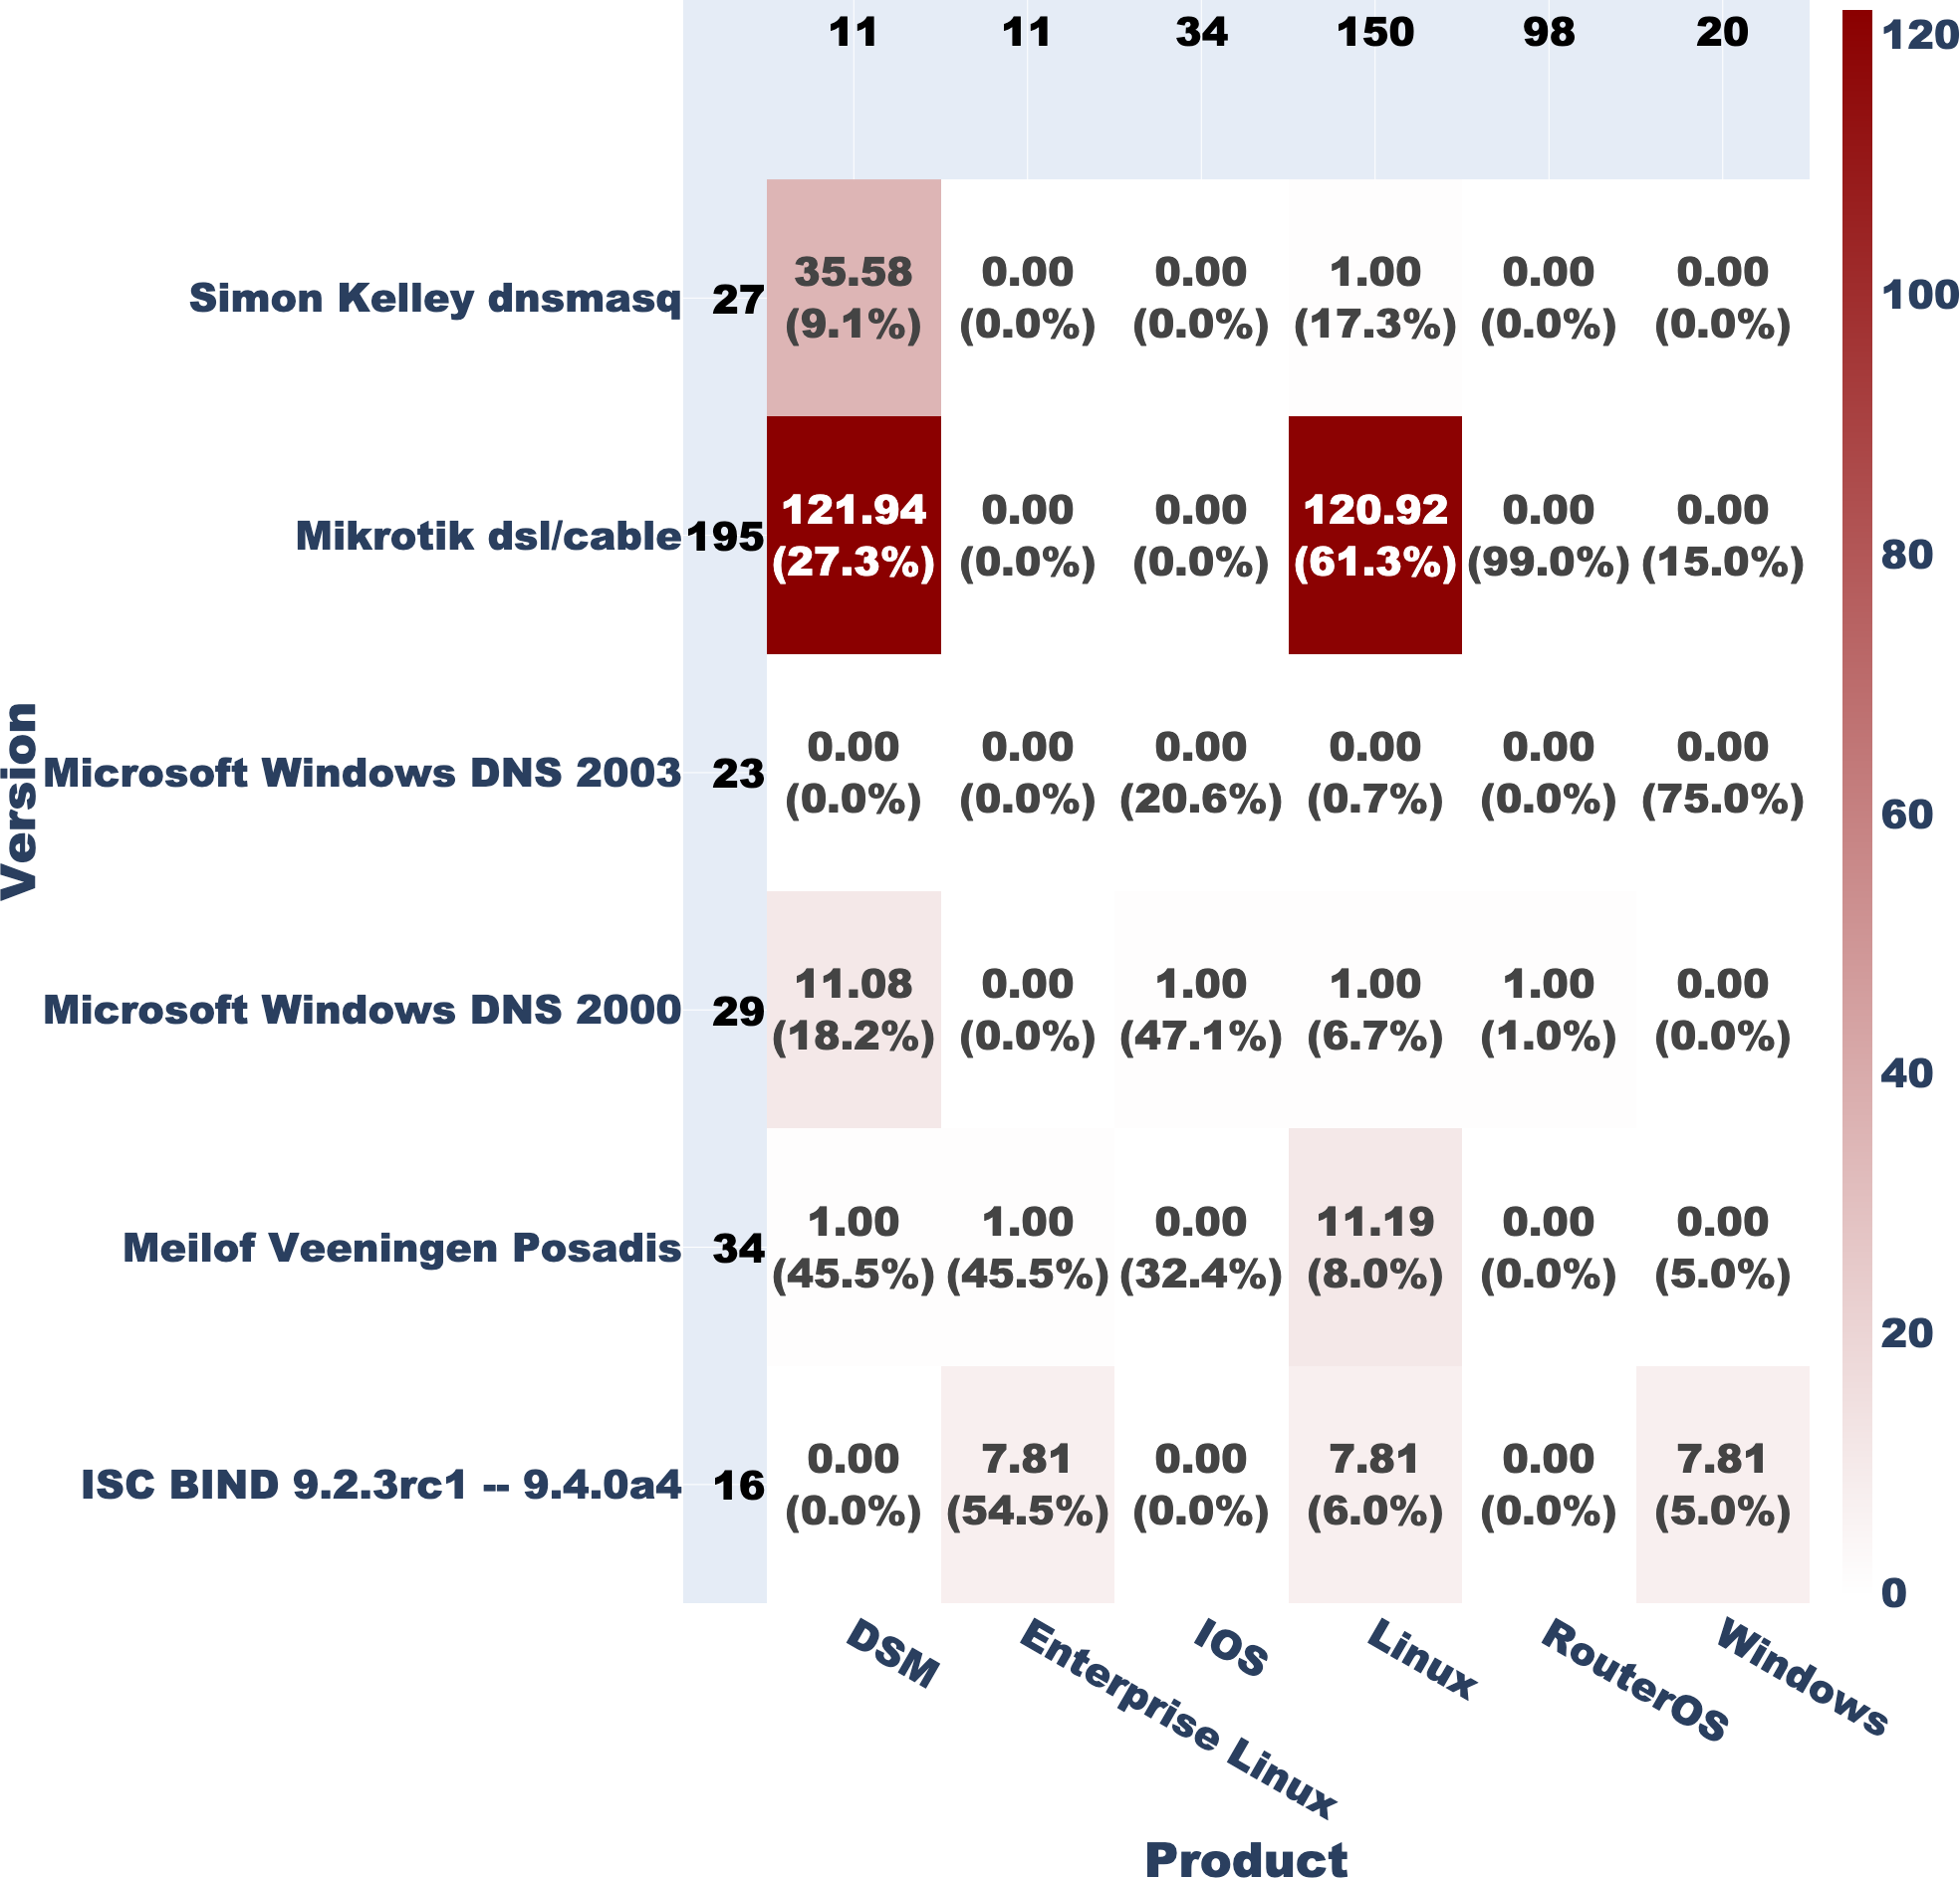
\includegraphics[width=\textwidth]{research paper/plots/filtered_Version_vs_Product_trim.png}
        \caption{Version against Product.}
        \label{fig:heatmap_version_product}
    \end{minipage}
    \hfill
    \begin{minipage}[t]{0.45\textwidth}
        \centering
        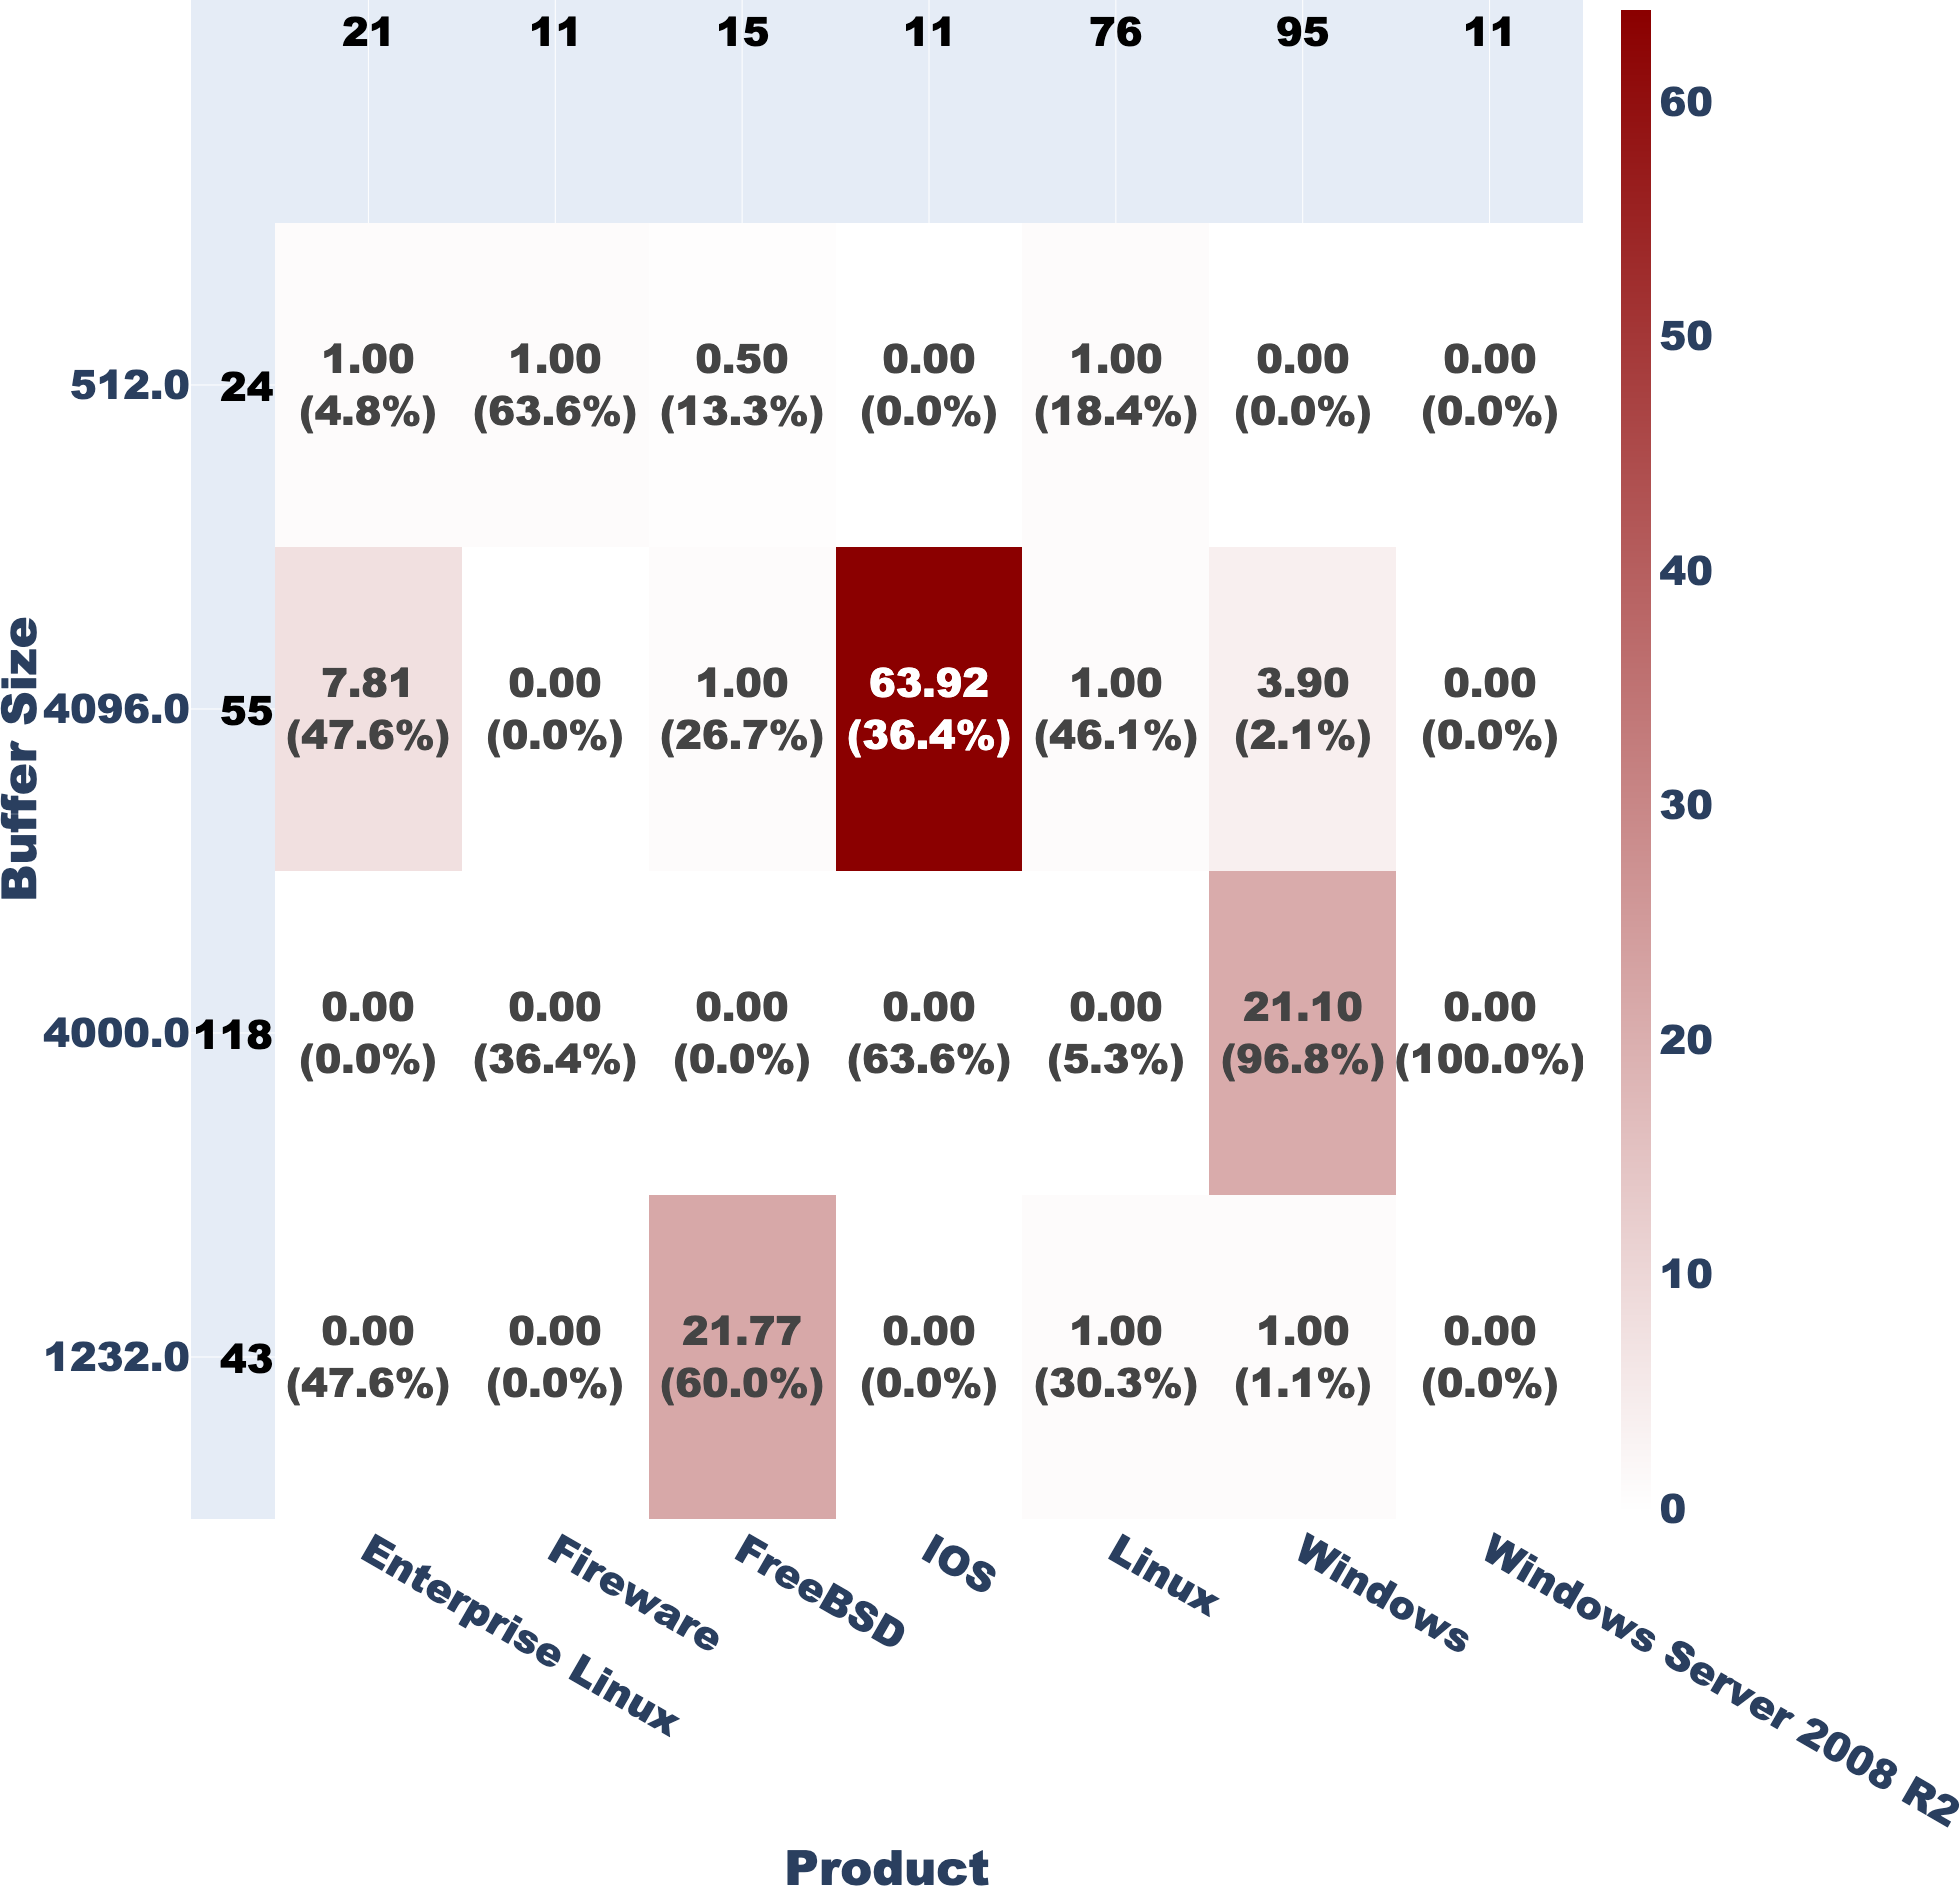
\includegraphics[width=\textwidth]{research paper/plots/filtered_Buffer Size_vs_Product_trim.png}
        \caption{Buffer Size against Product.}
        \label{fig:heatmap_buffer_product}
    \end{minipage}
\end{figure}


\section{Loopy attacks}
\label{appendix:loopy_attacks}
Below is a brief overview of the methodology created by~\cite{cispa-loopy} to find server pairs that are vulnerable to looping attacks. 

\looseness=-1 \textbf{Step 1.} In the first stage discovery packets are sent to all the servers go gather a complete set of responses. These could serve as the entry point to a traffic loop.  

\looseness=-1 \textbf{Step 2.} Since there could be many distinct responses (depending on the number of hosts), the second stage clusters the responses based on their semantics. Insignificant syntactic differences, such as the transaction ID (TXID), are ignored since they cannot influence a DNS response. In the end, several clusters will hold semantically equivalent responses. 

\looseness=-1 \textbf{Step 3.} With a similar reasoning as the second stage, in the third stage, random responses are sampled from each of the clusters. These will be the set of probes that will be sent again to each server. Sending all the initial responses to all the servers would have been both infeasible, due to the large number of initial responses, but also ineffective, since several packets from the same cluster are expected to have the same behaviour, and in turn, should themselves lead to the same response. The responses after this third stage also end up being clustered in the same way as the second stage.  

\looseness=-1 \textbf{Step 4.} With the information gathered in the third step, a loop graph can be formed. In this graph edges represent servers that reply to an input from one cluster with a response from the same or another cluster. Following this, a DFS is ran to find cycles with a length of at most 4.

\looseness=-1 \looseness=-1 \textbf{Step 5.} In the last stage, the loops that were identified previously are formally verified with a proxy. The proxy sits in between the two servers that are being tested and it forwards messages between the two. Once the proxy has forwarded enough messages, the two servers are validated as a loop pair. As this step required setting up a proxy, we have skipped it.

% \clearpage






% \section{Some further guidelines that go without saying (right?)}

% \begin{itemize}
% \item Read the manual for the Research Project. (See e.g.\ the instructions on the maximum length: less is more!)
% \end{itemize}

% \subsection{Reference use}
% \begin{itemize}
% \item use a system for generating the bibliographic information automatically from your database, e.g., use BibTex and/or Mendeley, EndNote, Papers, or \ldots
% \item all ideas, fragments, figures and data that have been quoted from other work have correct references
% \item literal quotations have quotation marks and page numbers
% \item paraphrases are not too close to the original
% \item the references and bibliography meet the requirements
% \item every reference in the text corresponds to an item in the bibliography and vice versa
% \end{itemize}

% \subsection{Structure}
% Paragraphs
% \begin{itemize}
% \item are well-constructed
% \item are not too long: each paragraph discusses one topic
% \item start with clear topic sentences
% \item are divided into a clear paragraph structure
% \item there is a clear line of argumentation from research question to conclusions
% \item scientific literature is reviewed critically
% \end{itemize}

% \subsection{Style}
% \begin{itemize}
% \item correct use of English: understandable, no spelling errors, acceptable grammar, no lexical mistakes 
% \item the style used is objective
% \item clarity: sentences are not too complicated (not too long), there is no ambiguity
% \item attractiveness: sentence length is varied, active voice and passive voice are mixed
% \end{itemize}

% \subsection{Tables and figures}
% \begin{itemize}
% \item all have a number and a caption
% \item all are referred to at least once in the text
% \item if copied, they contain a reference
% \item can be interpreted on their own (e.g. by means of a legend)
% \end{itemize}
